140. \begin{figure}[ht!]
\center{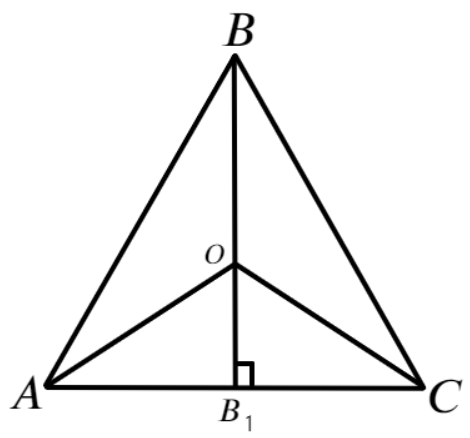
\includegraphics[scale=0.35]{g8-139.png}}
\end{figure}\\
Центр как вписанной, так и описанной окружности равностороннего треугольника --- это точка $O,$ являющаяся точкой пересечения как серединных перпендикуляров, так и биссектрис, медиан и высот (все эти линии в равностороннем треугольнике совпадают). Тогда $OB$ является радиусом описанной окружности, а $OB_1$ --- вписанной. Так как точка $O$ является ещё и точкой пересечения медиан, $BO=2OB_1,$ значит радиус вписанной окружности равен $8:2=4.$\newpage\noindent
